\chapter{Anhang}

\section{Projektmanagement}
Für die Projektorganisation kommen verschiedene Anwendungen und Hilfsmittel zur Anwendung. Im Folgenden werden die einzelnen Bereiche behandelt.

\subsection{Zeitplan}
Die Zeiterfassung ist in einem dafür vorbereiteten Excel File abgelegt. Folgende Meilensteine sind im Zeitplan festgelegt:

\begin{tabular}{p{2.1cm}p{7.5cm}r}
Projektstart & & 21.02.2012\\
Milestone 1 & \textit{RadioTour} Bestandesaufname Webanwendung & 05.03.2012\\
Milestone 2 & Plattform Entscheid gefällt & 12.03.2012\\
Milestone 3 & Features und Abgrenzung definiert und mit Heinzmann besprochen & 19.03.2012\\
Milestone 4 & Prototyp "'Rennsituation"` bei Heinzmann zum Testen übergeben & 09.04.2012\\
Milestone 5 & Dokumentation Teil Einleitung zur Review übergeben & 23.04.2012\\
Milestone 5.1 & Prototyp zum Testen an Heinzmann übergeben & 01.05.2012\\
Milestone 6 & Feature Freeze & 07.05.2012\\
Rennen & Berner Rundfahrt, Lyss & 12.05.2012\\
Milestone 7 & Code Freeze & 14.05.2012\\
Milestone 8 & Dokumentation Freeze & 21.05.2012\\
Milestone 9 & Abgabe komplett & 28.05.2012\\
Projektende & & 01.06.2012\\
Rennen & Gippingen (nach Abgabe) & 07.06.2012\\
Rennen & Tour de Suisse (nach Abgabe) & 09.-16.06.2012\\
\end{tabular}

Die Auswertung der Zeiterfassung zeigt deutlich mehr (Ist-) Arbeitsstunden an, als die in der Planung eingetragenen (Soll-) Stunden. Besonders bei der Implementierung ist oftmals mehr Zeit benötigt worden als ursprünglich geplant war. Weiter hat das Erstellen der Dokumentation  mehr Zeit in Anspruch genommen als erwartet. Der Projektzeitplan mit den vollständigen eingetragenen Arbeitsstunden ist in digitaler Form auf der beigelegten CD.

\subsection{Code Base und Issue Tracking}
Das Code Repository wurde auf Github\footnote{Github, \url{https://github.com/dstucki/RadioTour}, Aufgerufen am 11.05.2012.} erstellt und verwaltet. Dieses Repository ist öffentlich lesbar, jedoch kann nicht öffentlich darauf geschrieben werden.
\\
Nach der ersten Implementierungsphase sind die Probleme, Fehler und weiteren Features der Applikation im integrierten Issuetracker von Github erfasst. Die Issues sind einer der folgenden Kategorie zugeordnet:

\begin{itemize}
\item must
\item can
\item nice
\end{itemize}

Sämtliche "`must"' und "`can"' Issues wurden erfolgreich abgearbeitet. Offen geblieben ist ein einziges "`nice"' Issue. Dabei geht es um die Auswahl von Fahrern für die Zuweisung von Wertungen in einem Spezialklassement.




\section{Persönliche Berichte}

\subsection{Daniel Stucki}

\subsection{Florian Bentele}
Zu Beginn des Projekts war es für mich schwierig, den Arbeitsaufwand und die Erwartungen an mich abzuschätzen. Die Aufgabenstellung ist mehr als einen Anstoss zu verstehen und wird ständig weiter entwickelt und konkretisiert. Da wir aber schnell in die Thematik gefunden haben und unsere Ideen bei jeder Besprechung ein Stück weiter zu einem einsetzbaren Produkt führten, schwanden sämtliche Unsicherheiten. Besonders der Reiz, eine Applikation zu entwickeln, die den Anforderungen eines Live Sport Events entsprechen muss und in der Realität eingesetzt werden soll, führten zu einer hohen Einsatzbereitschaft und grosser Motivation. Ich hatte eine gewisse Verantwortung übernommen, die Applikation am Ende des Semesters funktionstüchtig abzuliefern. Weiter war es mir ein Anliegen, eine Arbeit im Bereich Mobile oder Web Applikationen zu erstellen. Mit diesem Projekt gelang es mir, einen tiefen Einblick in die Entwicklung von Android Applikationen zu erarbeiten.
\\
Die ersten Wochen verliefen dennoch harzig, da die Analyse der bestehenden Applikation sehr aufwändig und zeitintensiv war. Sämtliche Tools und das Projektmanagement wurden eingerichtet, die Aufgaben aufgeteilt. Bei der Implementierungsphase ging es dann sehr gut voran. Wir haben das Aufgabenumfeld in Teilprobleme aufgeteilt und diese dann abgearbeitet. In weiteren Projekten würde ich mehr Wert auf diese Aufteilung legen. Nach der fundamentalen Architektur, die in meinen Augen ein Prozess ist, bei dem das ganze Team dabei sein sollte, können die Features gut aufgeteilt werden. Nach dem Hauptteil der Implementierung hatten wir die einmalige Gelegenheit, unsere Applikation an einem Radrennen zu testen. Dies ermöglichte uns, ein echtes, unverfälschtes Feedback zu erhalten. Aus den Rückmeldungen konnten wir die Applikation weiter verbessern und für die Tour de Suisse bereit machen.  Im weiteren Verlauf versuchten wir, den bestehenden Code zu optimieren und verschönern (Refactoring). Da aber bis in der zweitletzen Woche des Projekts noch Features hinzukamen, war dies eher schwierig. Gegen Ende des Projekts kamen immer mehr Aufgaben im Bereich Dokumentation dazu. Aber auch diesen Teil konnten wir gut aufteilen.
\\
Die Zusammenarbeit mit Daniel Stucki hat optimal funktioniert. Ich konnte viel von seiner Erfahrung als Java Entwickler profitieren und wir haben die Herausforderung gemeinsam gemeistert. Insbesondere in der Entwicklung ist es für mich wichtig, Teilprobleme und deren Lösungsansätze mit einer involvierten Person diskutieren zu können. Ich freue mich, auch in der Bachelorarbeit mit Daniel Stucki zusammen arbeiten zu können.
\\
Aus diesem Projekt nehme ich diverse Erfahrungen mit, einerseits das Erlernte im Bereich der Android Programmierung, andererseits aus dem Projektmanagement und der Wichtigkeit einer möglichst genauen Zeitplanung. Auch die Meilensteine und der Feldtest sind gute Methoden, um den Projektverlauf möglichst zeitgerecht einzuhalten.


\section{Kriterienkatalog}
\label{ref:kriterien}
Hier sind die Kriterien

\section{Kaufempfehlung}
\label{ref:kaufempfehlung}

\section{UseCases der bisherigen Applikation}
\label{ref:usecases}
Im unten stehenden UseCase Diagramm (Abbildung \ref{fig:usecasediagram}) sind die primären UseCases aufgeführt. Nur der \textit{RadioTour Speaker} erfasst Daten in dieser Applikation und ist daher der einzige Aktor. Das System wird durch die \textit{RadioTour} Applikation abgebildet. Zur besseren Darstellung wurden einzelne UseCases vereinfacht oder zusammengefasst.
\begin{figure}[h1]
  \caption{UseCase Diagramm}
  \label{fig:usecasediagram}
  \begin{center}
    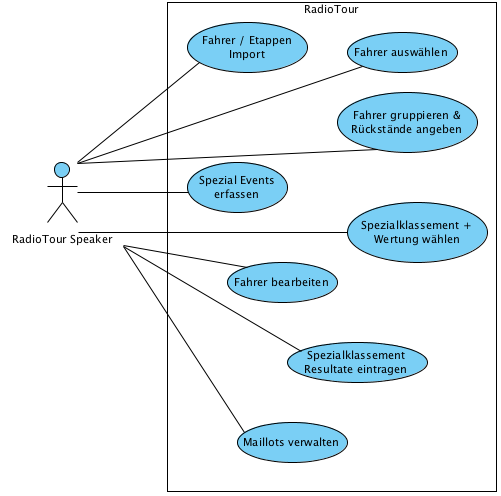
\includegraphics[scale=0.6]{05bericht/images/usecasediagram.png}
  \end{center}
\end{figure}

\begin{itemize}
\item \textbf{Fahrer auswählen}\\
Dem \textit{RadioTour Speaker} muss es möglich sein, einen oder mehrere Fahrer schnell auszuwählen. Die Fahrer werden im Auswahldialog bevorzugt durch ihre Startnummern dargestellt. An der Tour de Suisse besteht ein Team – nach Aussage von P. Heinzmann – aus 8 Fahrern. Um eine möglichst gute Übersicht zu gewährleisten, werden die Fahrer jeweils zeilenweise in deren Teams gruppiert. Ausgewählte Fahrer werden farblich hervorgehoben. Die Nummern der Fahrer, welche bereits Gruppen zugewiesen wurden, werden in Klammern dargestellt. Die Nummern ausgeschiedener Fahrer werden gestrichen dargestellt.

\begin{figure}[h!]
  \caption{Die Fahrerauswahlliste zur Gruppierung in der bisherigen Web Applikation}
  \begin{center}
    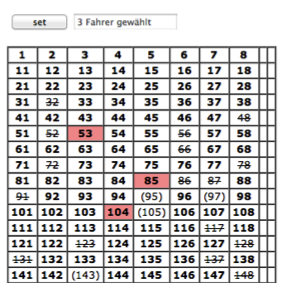
\includegraphics{05bericht/images/uc01_fahrerliste.png}
  \end{center}
\end{figure}

\item \textbf{Fahrer gruppieren}\\
Dem \textit{RadioTour Speaker} muss es möglich sein, die ausgewählten Fahrer in Gruppen zu organisieren. So kann er die ihm gemeldeten Rennsituationen mit Ausreissern, Verfolgern, Feld und Abgehängten darstellen.

\begin{figure}[H]
  \caption{Gruppierung in der bisherigen Web Applikation}
  \begin{center}
    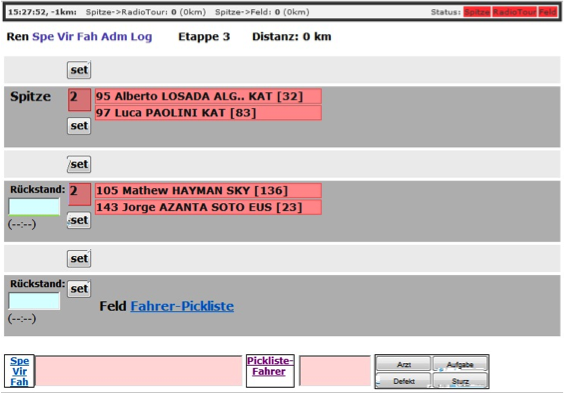
\includegraphics{05bericht/images/uc02_gruppen.png}
  \end{center}
\end{figure}

\item \textbf{Rückstände angeben}\\
Dem \textit{RadioTour Speaker} muss es möglich sein, für die Gruppen (siehe oben) ihre jeweiligen Zeitabstände relativ zur Spitze einzugeben. Falls vorhanden, sollen auch die mit dem TourLive GPS-System erfassten Zeitabstände Spitze-Feld eingeblendet werden.

\item \textbf{Spezial Events erfassen}\\
Dem \textit{RadioTour Speaker} muss es möglich sein, für ausgewählte Fahrer Spezialereignisse festzulegen. Dies sind beispielsweise Arztbesuch, Aufgabe, Defekt oder Sturz.
\begin{figure}[H]
  \caption{Die Spezialklassemente und Wertungen in der bisherigen Web Applikation}
  \begin{center}
    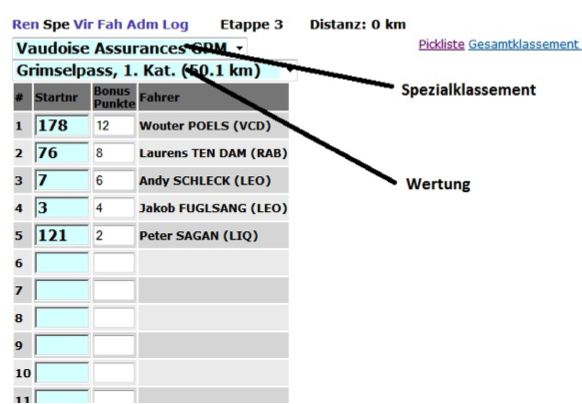
\includegraphics{05bericht/images/uc03_spezial.png}
  \end{center}
\end{figure}


\item \textbf{Spezialklassement und Wertung wählen}\\
Bei Mehretappenrennen werden typisch neben dem Gesamtklassement (schnellster Fahrer) mehrere Spezialklassemente (z.B. Bergpreis, Sprint, Punkteklassement) gewertet. Innerhalb der Etappen gibt es jeweils mehrere Stellen (Wertungen), an denen für die Spezialklassemente Punkte vergeben werden. Dem \textit{RadioTour Speaker} muss es möglich sein, die gewünschte Wertung zu einem der vorher erfassten Spezialklassemente auszuwählen.

\item \textbf{Spezialklassement Resultate eintragen}\\
Dem \textit{RadioTour Speaker} muss es möglich sein, für eine Wertung, welche er ausgewählt hat (siehe UC oben), die Ränge zur Wertung mit Fahrernummern zu verbinden, wodurch das Klassement generiert wird.

\item \textbf{Klassement anzeigen}\\
Das durch die eingetragene Wertung erstellte Klassement muss vom \textit{RadioTour Speaker} abgerufen werden können. Dort sollen alle Fahrer angezeigt werden, welche einen Punkterang in diesem Spezialklassement erreichten.

\item \textbf{Virtuelles Klassement}\\
Dem \textit{RadioTour Speaker} muss es möglich sein, ein aktuelles Klassement der Tour abzurufen und dieses nach bestimmten Kriterien zu sortieren. Die zurzeit möglichen Sortierkriterien sind:
\begin{itemize}
\item[-]Gruppen (zur Zeit des Aufrufs, nicht offiziell)
\item[-]Virtueller Rückstand (zur Zeit des Aufrufs, nicht offiziell)
\item[-]Zeitboni (zur Zeit des Aufrufs, nicht offiziell)
\item[-]Offizielle Zeit (zum Etappenende des Vortages, offiziell)
\item[-]Offizieller Rückstand (zum Etappenende des Vortages, offiziell)
\end{itemize}

\begin{figure}[h!]
  \caption{Virtuelles Klassement in der bisherigen Applikation}

  \begin{center}
    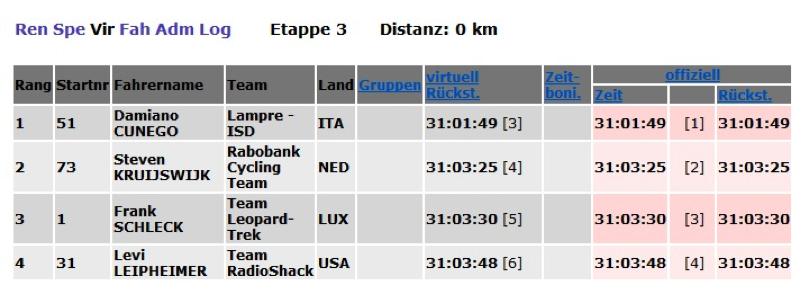
\includegraphics{05bericht/images/uc05_virtuell.png}
  \end{center}
\end{figure}

\item \textbf{Fahrerliste anschauen}\\
Dem \textit{RadioTour Speaker} muss es möglich sein, die aktuelle Fahrerliste anzuschauen. Die Fahrerliste ist nach Startnummern aufsteigend sortiert. (Die Startnummern werden in Mehretappenrennen so vergeben, dass die Fahrer eines Teams aufeinanderfolgende Startnummern erhalten.)

\begin{figure}[h!]
  \caption{Die Fahrerliste mit den Informationen zum Status der Fahrer}
  \begin{center}
    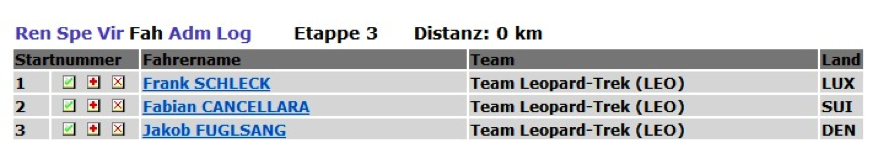
\includegraphics{05bericht/images/uc06_fahrerliste.png}
  \end{center}
\end{figure}

\item \textbf{Fahrer de- bzw. aktivieren}\\
Dem \textit{RadioTour Speaker} muss es möglich sein, einzelne Fahrer zu deaktivieren bzw. wieder zu aktivieren. Der Grund der Deaktivierung soll auch später noch nachvollziehbar sein. Es soll möglich sein, den Grund für die Deaktivierung anzugeben (z.B. ausgeschieden, nicht gestartet, andere).
Eine so vorgenommene Deaktivierung eines Fahrers muss durch den \textit{RadioTour Speaker} rückgängig gemacht werden können.

\item \textbf{Fahrerdetails bearbeiten}\\
Dem \textit{RadioTour Speaker} muss es möglich sein, einen Fahrer aus der Fahrerliste auszuwählen, um seine Details anzuschauen und auch zu bearbeiten. 

\item \textbf{Statistik}\\
Dem \textit{RadioTour Speaker} muss es möglich sein, in seinem Admin-Bereich eine kurze und prägnante textbasierte Statistik zu erhalten, aus welcher er auf einen Blick sieht, wie viele Fahrer in der Datenbank sind und welche davon aktiv sind. Darüber hinaus die Anzahl Gruppen, Spezialklassemente, Wertungen und vergebene Punkte.

\item \textbf{Import Fahrerliste}\\
Nach jedem Renntag ( = Etappe), wird in die \textit{RadioTour} Applikation eine neue Fahrerliste mit den aktuellen offiziellen Zeiten importiert. Deshalb muss es dem \textit{RadioTour Speaker} möglich sein, die aktuellen Zeiten zu importieren. Derzeit sind für den Import der Daten verschiedene Importverfahren implementiert, wie dies im Screenshot ersichtlich ist.

\item \textbf{Erfassung Spezialklassemente}\\
Dem \textit{RadioTour Speaker} muss es möglich sein, Spezialklassemente zu erfassen. Diese Erfassungen werden vor der Tour de Suisse getätigt, weshalb ein Import hier nicht notwendig ist.

\item \textbf{Speicherung Maillots}\\
Dem \textit{RadioTour Speaker} muss es möglich sein, die Belegung der 4 verschiedenen Maillots anzugeben und zu sichern. Folgende Maillots werden an der Tour de Suisse vergeben:

\begin{center}
  \begin{tabular}{ l | l  }
    \hline
    Name & Farbe \\ \hline
    \hline
    Bergpreis & Rot-Weiss \\ \hline
    Gesamtklassement & Gelb \\ \hline
    Neo-Profi & Weiss \\ \hline
    Punkte & Grün\\

    \hline
  \end{tabular}
\end{center}


\item \textbf{Daten exportieren}\\
Dem \textit{RadioTour Speaker} muss es möglich sein, die Spezialklassemente, Wertungen, Fahrer nicht nur zu erfassen, importieren und bearbeiten, sondern auch als *.csv zu exportieren. Dabei werden einfach alle mit dem gewünschten Export assoziierten Infos in das exportierte *.csv geschrieben.

\end{itemize}

\section{Usability Test}
\label{ref:usability}
Mit David Loosli, dem \textit{RadioTour Speaker} an der Berner Rundfahrt 2012, wurde am 11.05.2012 ein Testlauf mit dem Tablet durchgeführt. Dabei wurde an einem vorgängigen Treffen folgende fiktive Situation durchgespielt, um den Umgang mit der Applikation zu erklären.

\begin{itemize}
\item Alle Fahrer sind importiert und das Rennen beginnt jetzt
\item Rennzeit wird gestartet
\item Fahrer 4 \& 17 von Beginn an, an der Spitze
\item Bereits 1:07 Vorsprung
\item 31 hat ein defektes Rad und muss raus
\item Der Vorsprung erhöht sich auf 2:19
\item 8, 83 \& 34 fallen hinter das Feld mit einem Rückstand von 4:31
\item 8 kann wieder etwas aufholen und löst sich vom Feld, Rückstand nur noch 3:45
\item 7 \& 11 sind der Spitze an den Fersen mit einem Rückstand von 0:42
\item 13 rückt zu 7\&11 auf
\item 41 ist verletzt und muss zum Arzt
\item Chrono1 ist beim Ortseingang Lyss, ... Jetzt. Stoppuhr
\item 37 49 45 rücken in die Verfolgergruppe vor
\item Wir sind beim Ortseingang Lyss, Stoppuhr
\item 19 \& 71 fallen eine Gruppe zurück
\item 11 kommt an die Spitze
\item Rennzeit wird korrigiert auf 05:11
\item 71 kann nicht mehr und hat aufgegeben
\item Rückstand vom Feld erhöht sich um 20 s
\item Info kommt rein, dass die 3 (Marcel Aregger), eigentlich Michael Aregger heisst
\item Aregger (3) kann zur die Spitze aufschliessen
\item Hinter dem Feld bildet sich eine neue Gruppe mit den Fahrern 19, 24, \item 51 \& 36. Rückstand 3:11
\item 19 stürzt
\item 24 Rückt wieder ins Feld auf
\item 51 und 36 fallen weiter in die nächste Gruppe zurück
\item 52 rückt zur Spitze vor
\item Rückstand Feld neu 1:30
\end{itemize}

\subsection{Auswertung und Feedback}
Alle Änderungen konnten durch David Loosli erfasst werden. Der erste Eindruck war sehr gut, folgende Vorschläge wurden aufgenommen und in der Weiterentwicklung umgesetzt:
\begin{itemize}
\item Beim TimePicker sind die Nummern zu klein dargestellt, es benötigt keine Stunden
\item Fahrer werden nur bei "`Aufgabe"'  und "`nicht erschienen"' ausgegraut und durchgestrichen, bei "`Arzt"', "`Sturz"' und "`Defekt"' werden die Fahrernummern eingefärbt
\item ein Fahrer kann die folgenden Status haben
\begin{itemize}
\item im Rennen / aktiv
\item nicht gestartet
\item ausgeschieden
\end{itemize}
\item Tablet darf nicht verdunkeln, falls es einen Moment nicht verwendet wird (Hardwareeinstellung)
\item Rennkilometer muss editierbar sein. Weiter sind die noch zu fahrenden Kilometer anzuzeigen
\item Rennzeit und Kilometer sind nach einem Absturz der Applikation noch verfügbar
\end{itemize}
